\documentclass[12pt,a4paper]{article}

\usepackage[a4paper,top=1in,bottom=1in,left=1in,right=1in]{geometry}
\usepackage{graphicx}
\usepackage{float}
\usepackage{amsmath}
\usepackage{newtxtext}
\usepackage{newtxmath}
\usepackage{xcolor}
\usepackage{listings}
\usepackage{caption}
\usepackage{parskip}
\usepackage[hidelinks]{hyperref}

\pagestyle{plain}
\setlength{\parindent}{0pt}
\setlength{\parskip}{0.75em}
\linespread{1.06}

\lstdefinestyle{pythoncode}{
    language=Python,
    basicstyle=\ttfamily\footnotesize,
    keywordstyle=\bfseries\color{blue!60!black},
    commentstyle=\itshape\color{green!40!black},
    stringstyle=\color{red!50!black},
    numbers=none,
    showstringspaces=false,
    breaklines=true,
    columns=fullflexible,
    keepspaces=true,
    frame=single,
    xleftmargin=1em,
    xrightmargin=0.5em,
    framexleftmargin=0.8em,
    framexrightmargin=0.5em,
    aboveskip=1em,
    belowskip=1em,
    lineskip=2pt,
    rulecolor=\color{black!35},
    backgroundcolor=\color{black!3},
    tabsize=4
}

\begin{document}

\begin{titlepage}
\thispagestyle{empty}
\centering

\vspace*{0.05in}

{\Large\bfseries TRIBHUVAN UNIVERSITY\par}
\vspace{0.16in}
{\large INSTITUTE OF ENGINEERING\par}
\vspace{0.12in}
{\large PURWANCHAL CAMPUS\par}

\vspace{0.5in}

\includegraphics[width=1.55in]{../assets/tu-logo.jpg}

\vspace{0.55in}
{\Large\bfseries DSAP ASSIGNMENT - 1\par}

\vspace{0.3in}
{\Large\bfseries IMPLEMENTATION OF BASIC SIGNALS\par}

\vspace{0.5in}
{\large\bfseries BY\par}

\vspace{0.25in}
{\large Tilak Thapa [PUR079BCT094]\par}

\vfill

{\normalsize DEPARTMENT OF ELECTRONICS AND COMPUTER ENGINEERING\par}
\vspace{0.14in}
{\normalsize PURWANCHAL CAMPUS\\ DHARAN, SUNSARI\par}

\vspace{0.3in}
{\normalsize 18 JUNE\par}

\end{titlepage}

\clearpage
\pagenumbering{arabic}
\setcounter{page}{1}

\section*{OBJECTIVE}

The objective of this assignment is to write a Python program that implements the required elementary signals. Each signal is implemented using a separate function and demonstrated graphically.

\section*{SOFTWARE AND LIBRARIES USED}

\begin{itemize}
    \item Subject: Digital Signal Analysis and Processing

    \item Programming language: Python
    \item Libraries used: NumPy and Matplotlib
    \item Purpose of NumPy: numerical signal generation
    \item Purpose of Matplotlib: graphical representation of signals
\end{itemize}

\section*{THEORY AND IMPLEMENTATION}

The following subsections describe each implemented signal. The code snippets show the separate Python functions used for signal generation. NumPy is imported as \texttt{np} in the program.

\subsection*{1. UNIT IMPULSE SIGNAL}

The unit impulse signal has value 1 at the origin and 0 elsewhere.

\[
\begin{aligned}
\delta[n] = 1 \text{ for } n = 0 \\
\delta[n] = 0 \text{ for } n \neq 0
\end{aligned}
\]

\begin{lstlisting}[style=pythoncode]
# Input: n, sample index array
# Output: unit impulse values
def unit_impulse(n):
    signal = np.where(n == 0, 1, 0)
    return signal
\end{lstlisting}

The function returns a NumPy array containing 1 only at n = 0.

\subsection*{2. UNIT STEP SIGNAL}

The unit step signal changes from 0 to 1 at the origin.

\[
\begin{aligned}
u[n] = 1 \text{ for } n \geq 0 \\
u[n] = 0 \text{ for } n < 0
\end{aligned}
\]

\begin{lstlisting}[style=pythoncode]
# Input: x, sample index array
# Output: unit step values
def unit_step_function(x):
    signal = np.where(x >= 0, 1, 0)
    return signal
\end{lstlisting}

The function returns a NumPy array with 0 before the origin and 1 from the origin onward.

\subsection*{3. UNIT RAMP SIGNAL}

The unit ramp signal increases linearly after the origin and remains zero before the origin.

\[
\begin{aligned}
r[n] = n \text{ for } n \geq 0 \\
r[n] = 0 \text{ for } n < 0
\end{aligned}
\]

\begin{lstlisting}[style=pythoncode]
# Input: x, sample index array
# Output: unit ramp values
def unit_ramp_function(x):
    signal = np.where(x >= 0, x, 0)
    return signal
\end{lstlisting}

The function returns a NumPy array that is zero before n = 0 and equal to n after n = 0.

\subsection*{4. COMPLEX EXPONENTIAL SIGNAL}

A complex exponential signal contains real and imaginary components. It can show oscillation and growth or decay depending on the value of the exponential factor.

\[
x[n] = e^{(a + j\omega)n}
\]

\begin{lstlisting}[style=pythoncode]
# Input: n, decay factor a, angular frequency omega
# Output: complex exponential values
def complex_exponential_function(n, a, omega):
    signal = np.exp((a + 1j * omega) * n)
    return signal
\end{lstlisting}

The function returns a complex NumPy array containing real and imaginary signal values.

\subsection*{5. REAL EXPONENTIAL INCREASING SIGNAL}

A real exponential signal increases when the exponent factor is positive.

\[
x[n] = e^{an}
\]

\begin{lstlisting}[style=pythoncode]
# Input: n, positive growth factor a
# Output: increasing real exponential values
def real_exponential_function_increasing(n, a):
    signal = np.exp(a * n)
    return signal
\end{lstlisting}

The function returns a NumPy array whose values increase exponentially.

\subsection*{6. REAL EXPONENTIAL DECREASING SIGNAL}

A real exponential signal decreases when the exponent factor is negative.

\[
x[n] = e^{-an}
\]

\begin{lstlisting}[style=pythoncode]
# Input: n, positive decay factor a
# Output: decreasing real exponential values
def real_exponential_function_decreasing(n, a):
    signal = np.exp(-a * n)
    return signal
\end{lstlisting}

The function returns a NumPy array whose values decrease exponentially.

\subsection*{7. RECTANGULAR SIGNAL}

A rectangular signal has constant amplitude for a fixed duration and zero value outside that duration.

\[
\begin{aligned}
x[n] = 1 \text{ for } 0 \leq n < W \\
x[n] = 0 \text{ otherwise}
\end{aligned}
\]

\begin{lstlisting}[style=pythoncode]
# Input: n, rectangular width
# Output: rectangular signal values
def rectangular_signal(n, width):
    signal = np.where((n >= 0) & (n < width), 1, 0)
    return signal
\end{lstlisting}

The function returns a NumPy array with value 1 inside the selected width and 0 elsewhere.

\subsection*{8. SAWTOOTH SIGNAL}

A sawtooth signal increases linearly during one period and then drops back to the starting value.

\[
x[n] = (n \bmod T) / T
\]

\begin{lstlisting}[style=pythoncode]
# Input: n, signal period
# Output: sawtooth signal values
def sawtooth_signal(n, period):
    signal = (n % period) / period
    return signal
\end{lstlisting}

The function returns a NumPy array containing one repeated rising ramp per period.

\subsection*{9. PCM SIGNAL}

Pulse Code Modulation represents an analog signal using discrete quantized levels. In this assignment, a sine wave is quantized into 16 levels.

\[
q[n] = \operatorname{round}\left(((x[n] + 1) / 2) \times (L - 1)\right)
\]

\begin{lstlisting}[style=pythoncode]
# Input: n, quantization levels
# Output: quantized PCM signal values
def pcm_signal(n, levels):
    analog_signal = np.sin(2 * np.pi * n / 20)
    quantized_indices = np.round(((analog_signal + 1) / 2) * (levels - 1))
    signal = (2 * quantized_indices / (levels - 1)) - 1
    return signal
\end{lstlisting}

The function returns a NumPy array containing quantized sine wave samples.

\section*{PROGRAM SUMMARY}

The program defines a separate Python function for each required signal. The total number of samples used is \(n = 100\). The unit impulse, unit step, and unit ramp signals are displayed over the range \(-50\) to \(49\). The complex exponential signal uses \(a = -0.02\) and \(\omega = 0.2\). The increasing and decreasing real exponential signals use \(a = 0.05\). The rectangular signal uses width \(20\), the sawtooth signal uses period \(20\), and the PCM signal uses \(16\) quantization levels.

All signals are calculated using NumPy arrays and plotted using Matplotlib. The output graph clearly shows the nature of each implemented signal.

\section*{OUTPUT}

The combined output image below shows all implemented signals in one view. The unit impulse contains one non-zero sample at the origin. The unit step changes from zero to one at the origin. The unit ramp grows linearly after zero. The complex exponential shows oscillating real and imaginary values with decreasing amplitude. The real exponential increasing signal grows with sample index, while the real exponential decreasing signal gradually approaches zero. The rectangular signal stays high for the selected width. The sawtooth signal repeats after each selected period. The PCM signal shows a quantized sinusoidal waveform.

\begin{figure}[H]
    \centering
    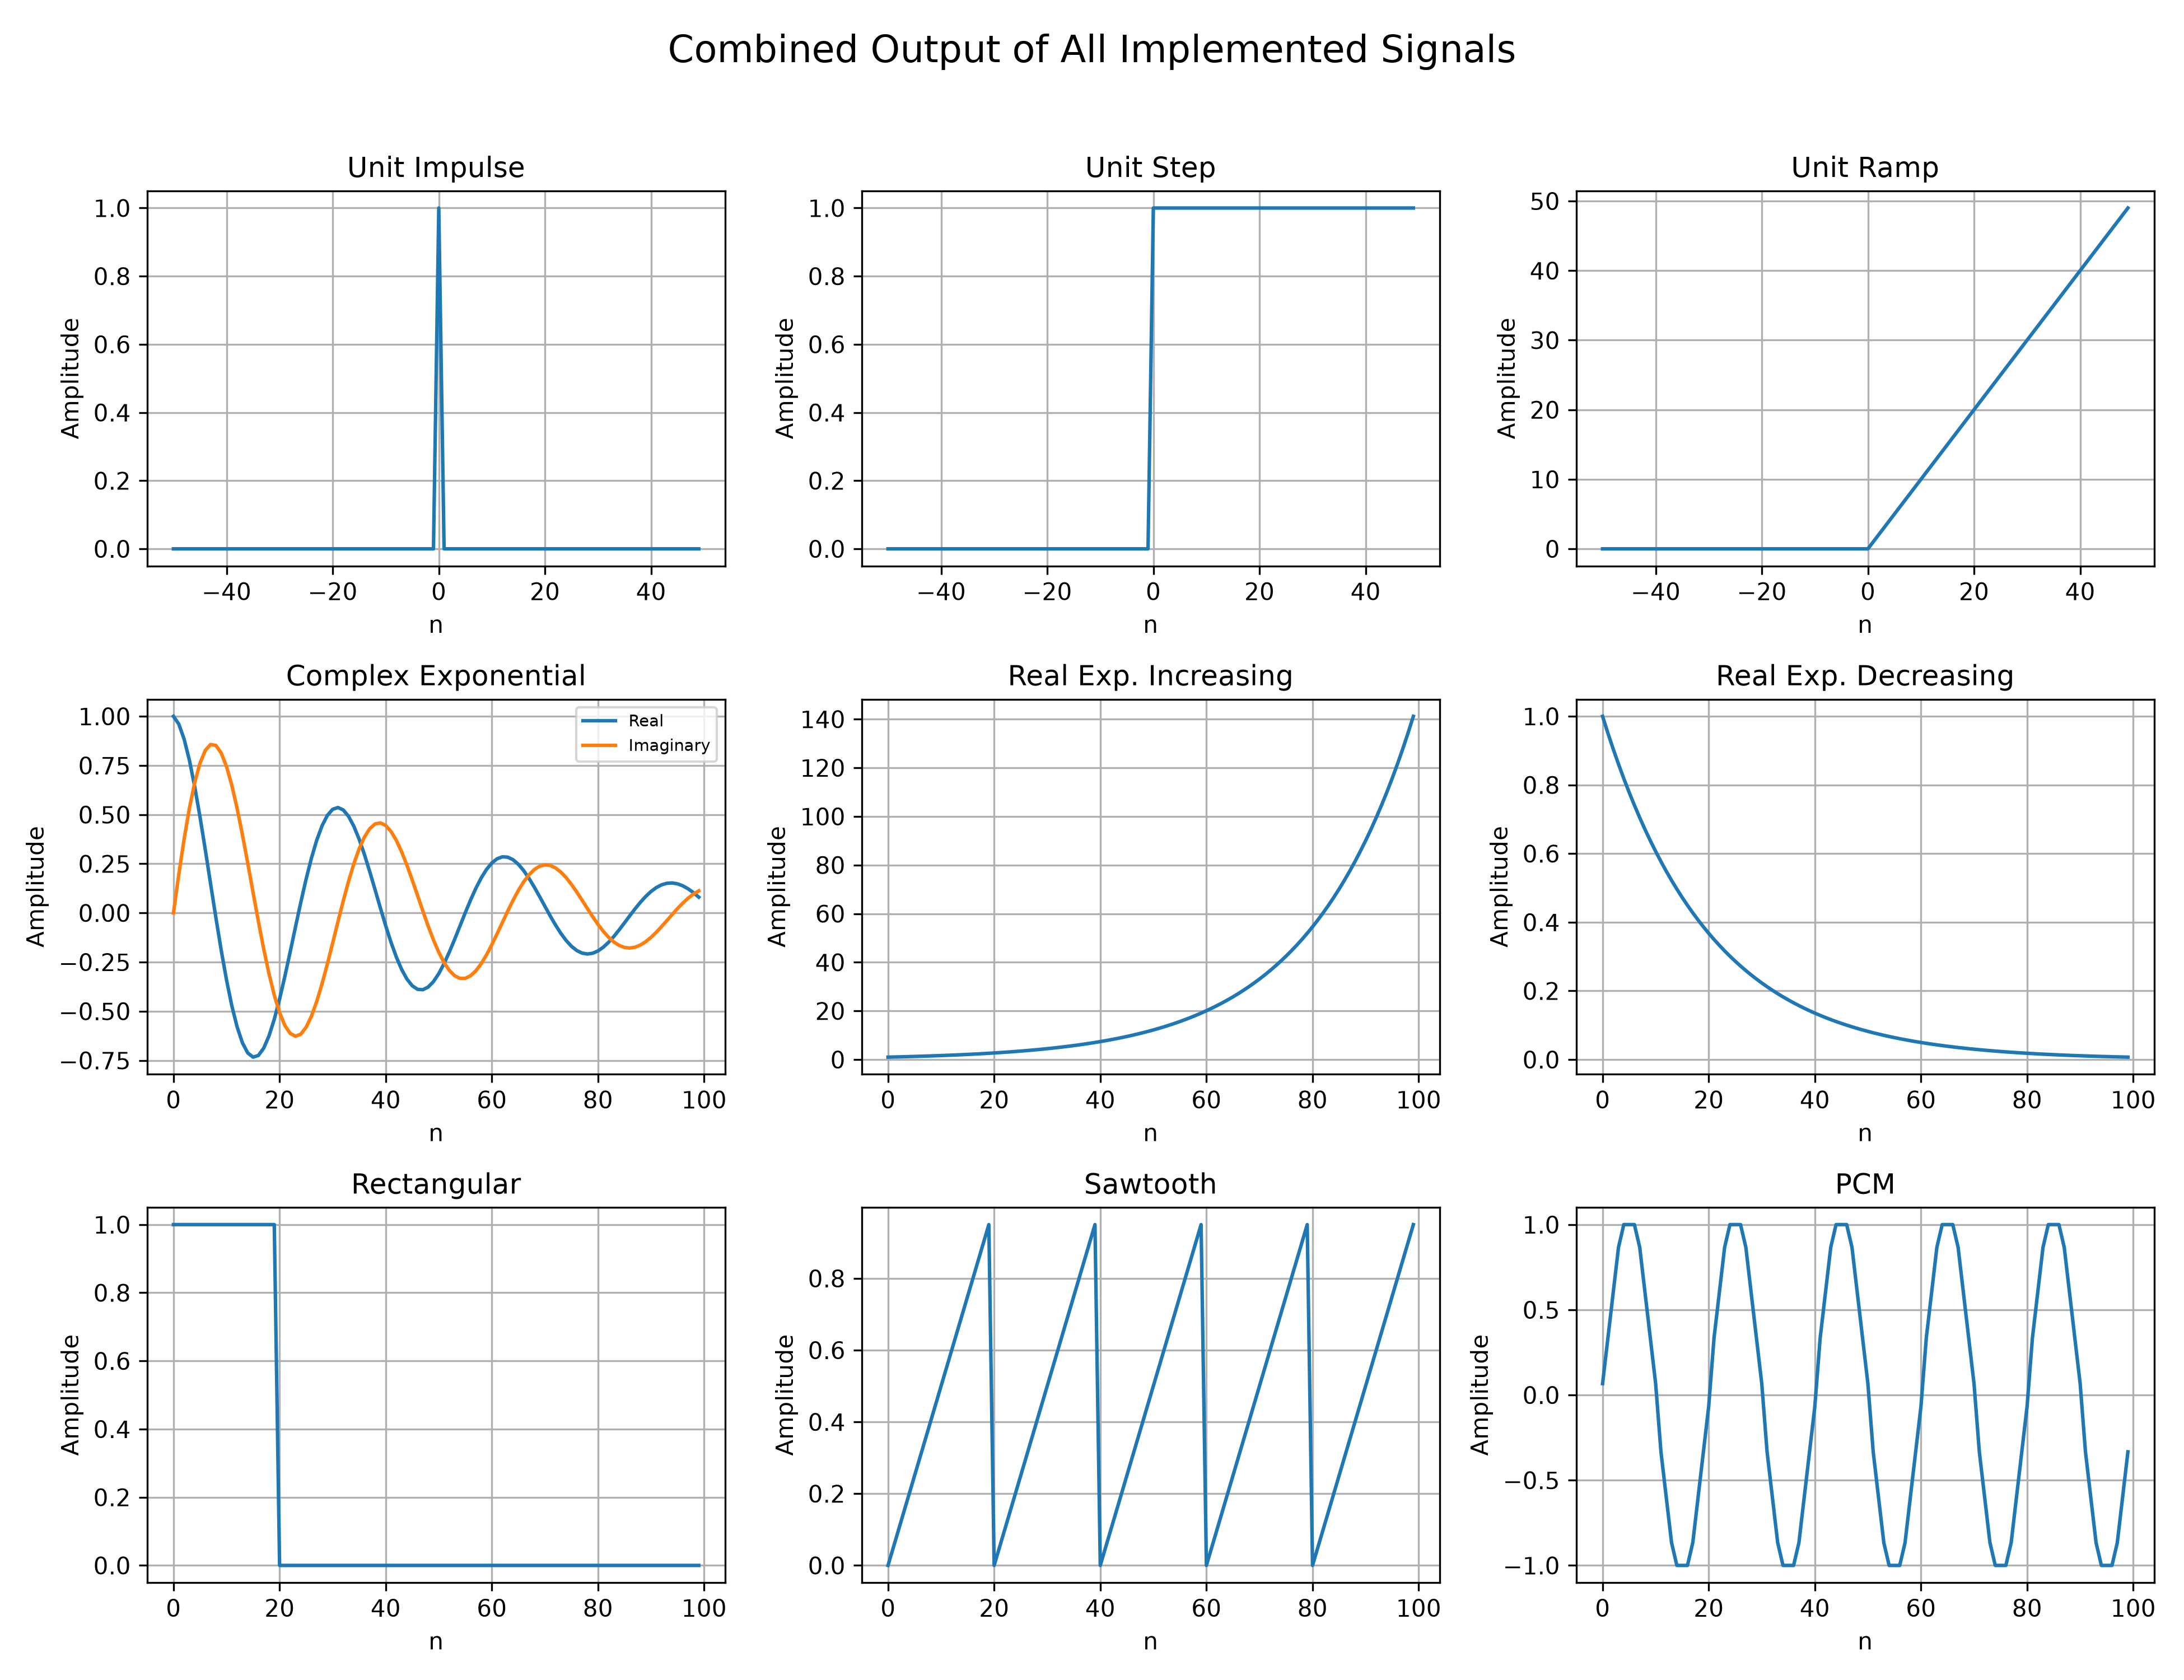
\includegraphics[width=0.96\textwidth]{combined_signals.png}
    \caption{Combined output of all implemented signals}
\end{figure}

\section*{RESULT AND DISCUSSION}

The output successfully demonstrates all required signals. The unit impulse contains a single non-zero sample at the origin. The unit step changes from 0 to 1 at zero, while the unit ramp grows linearly after zero. The complex exponential plot shows separate real and imaginary components with decreasing amplitude. The real exponential plots show both increasing and decreasing behavior. The rectangular signal remains high for the selected width and then becomes zero. The sawtooth signal repeats after every selected period, and the PCM signal shows a quantized sinusoidal waveform using 16 discrete levels.

\section*{CONCLUSION}

The assignment was completed by implementing each required signal in a separate Python function and displaying the output graphically. The result shows the basic behavior of impulse, step, ramp, complex exponential, real exponential, rectangular, sawtooth, and PCM signals.

\end{document}
